\documentclass[11pt]{article}
\usepackage[utf8]{inputenc}
%\usepackage[latin1]{inputenc}
\usepackage[spanish]{babel}
\usepackage{anysize}
\usepackage{graphicx} 
\usepackage{amsmath}
%\numberwithin{equation}{list}
\marginsize{1cm}{2cm}{0cm}{2cm}  
\title{Tarea 3 - Ecuaciones diferenciales ordinarias \\ \begin{large}Curso de F\'{i}sica Computacional\end{large}}
\author{M. en C. Gustavo Contreras May\'{e}n}
\date{ }
\begin{document}
\maketitle
\begin{enumerate}
\item En la figura (\ref{fig:sistemamecanico}) se muestra un sistema de tres masas. Los desplazamientos de estas tres masas satisfacen las ecuaciones dadas por
\begin{eqnarray} 
M_{1} y^{''}_{1} + B_{1}y^{'}_{1}+K_{1}y_{1} - B_{1}y^{'}_{2}-K_{2}y_{2} & = & F_{1}(t) \nonumber \\
-B_{1}y{'}_{1} - K_{1}y_{1} + M_{2}y^{''}_{2} + B_{1}y^{'}_{2} +(K_{1}+K_{2})y_{2} - K_{2}y_{3} & = & 0 \label{eq:sistema3masas} \\
-K_{2}y_{2}+M_{3}y^{''}_{3} + B_{2}y^{'}_{3} + (K_{2}+K_{3})y_{3} & = & F_{3}(t) \nonumber
\end{eqnarray}
Las constantes y condiciones iniciales son
\begin{tabbing}
$K_{1} = K_{2} = K_{3} = 1$ \hspace{5.5cm} \= (constantes de los resortes, kgm/$s^{2}$) \\
$M_{1} = M_{2} = M_{3} = 1$ \> (masa, kg) \\
$F_{1}(t) = 1, F_{3}(t) = 0$ \> (fuerza, N) \\
$B_{1} = B_{2} =0.1$ \> (coeficientes de amortiguamiento, kg/s) \\
$y_{1}=0 = y^{'}_{1}(0) =y_{2}=0 = y^{'}_{2}(0) = y_{3}=0 = y^{'}_{3}(0)$ \> (condiciones iniciales)
\end{tabbing}
\begin{figure}[!h]
	\centering	
	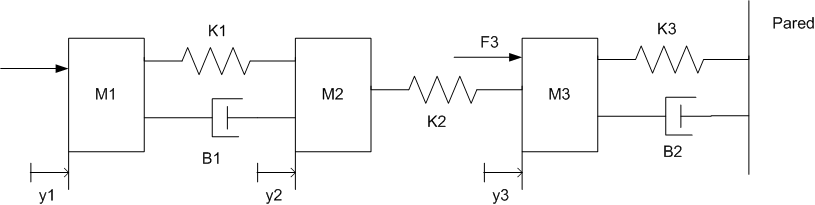
\includegraphics[scale=0.4]{Tarea3_01.png}
	\label{fig:sistemamecanico}
	\caption{Sistema de masas resortes}
\end{figure}
Resuelve y grafica las ecuaciones anteriores mediante RK4, para $0 \leq t \leq 30$ segundos y $h=0.1$ \\
Hint: Definiendo
\[ y_{4} = y^{'}_{1}, \hspace{1cm} y_{5} = y^{'}_{2}, \hspace{1cm} y_{6} = y^{'}_{3} \]
La ecuaci�n (\ref{eq:sistema3masas}) se escribe como un conjunto de seis EDO de primer orden, de la siguiente manera:
\begin{eqnarray}
y^{'}_{1} & = & y_{4} \\
y^{'}_{2} & = & y_{5} \\
y^{'}_{3} & = & y_{6} \\
y^{'}_{4} & = & \left[ -B_{1}y_{4} - K_{1}y_{1} + B_{1}y_{5} + K_{2}y_{2} + F_{1} \right] / M_{1} \\
y^{'}_{5} & = & \left[ B_{1}y_{4} + K_{1}y_{1} - B_{1}y_{5} - \left( K_{1}+K_{2} \right) y_{2} + K_{2}y_{3} \right] / M_{2}\\
y^{'}_{6} & = & \left[ K_{2}y_{2} - B_{2}y_{6} - \left( K_{2}+ K_{3} \right)y_{3} + F_{3} \right] / M_{3}
\end{eqnarray}
\item Una varilla de 1 m de longitud colocada en el vac�o, se calienta mediante una corriente el�ctrica aplicada a la misma. La temperatura en los extremos se fija en 273 K. El calor se disipa de la superficie mediante la transferencia de calor por radiaci�n hacia el ambiente, cuya temperatura es 273 K. Con las siguientes constantes, determina la distribuci�n de temperatura en la direcci�n del eje.
\begin{tabbing}
k = 60 W/mK \hspace{2.5cm} \= (conductividad t�rmica) \\
Q = 50 W/m \> (tasa de generaci�n de calor por unidad de longitud de barra) \\
$\sigma$= 5.67 $\times 10^{-8}$ W/$m^{2}K^{4}$ \> (constante de Stefan-Boltzamann) \\
A= 0.0001 $m^{2}$ \> (�rea de la secci�n transversal) \\
P = 0.01 m \> (per�metro de la varilla)
\end{tabbing}
La ecuaci�n de conducci�n de calor en la direcci�n del eje x es
\begin{equation} \label{eq:prob2}
-Ak \frac{d^{2}}{dx^{2}} T + P \sigma \left( T^{4} - 273^{4} \right) = Q \hspace{1.5cm} 0 < x < 1.0 
\end{equation}
con las condiciones de frontera dadas por
\[ T(0) = T(1.0) = 273 K \]
donde T es la temperatura en grados Kelvin.
\\ Este es un problema con condiciones en la frontera (espec�ficadas en $x=0$ y $x=1$), pero se puede resolver como un problema de condici�n inicial sobre la base de prueba y error. Definimos $y_{1}$ y $y_{2}$ como
\begin{eqnarray}
y_{1}(x) & = & T(x)\\
y_{2}(x) & = & T^{'}(x)
\end{eqnarray}
La ecuaci�n (\ref{eq:prob2}) se puede re-escribir como un conjunto de dos EDO de primer orden como
\begin{eqnarray}
y^{'}_{1} & = & y_{2} \\
y^{'}_{2} & = & \frac{P}{Ak} \sigma (y^{4} - 273^{4}) - \frac{Q}{kA}
\end{eqnarray}
Solo se obtiene una condici�n inicial $y_{1}=273$, a partir de las condiciones de frontera ($y_{2}$  no se conoce). Por ello, resolvemos la ecuaci�n (\ref{eq:prob2}) con valores de prueba para $y_{2}(0)$, hasta satisfaceer la condici�n de la frontera para el extremo derecho $y_{1}(1)=273$. Este enfoque se llama \textit{m�todo de disparo}.
\item Se dispara un proyectil al aire con un �ngulo de $45^{\circ}$ con respecto al suelo, con $u=v=150 m/s$, donde $u$ y $v$ son las velocidades horizontal y vertical, respectivamente. Las ecuaciones de movimiento est�n dadas por
\begin{eqnarray*}
u^{'} & = & -c Vu, \hspace{1.5cm} u(0)=150 m/s \\
v^{'} & = & -g - cVv, \hspace{1.5cm} v(0)=150 m/s
\end{eqnarray*}
donde $u$ y $v$ son funciones del tiempo, $u=u(t)$ $y v=v(t)$ y
\begin{eqnarray*}
V & = & \sqrt{u^{2} + v^{2}} \\
c & = & 0.005 \hspace{2cm} \text{(coeficiente de arrastre)} \\
g & = & 9.9 m/s^{2}
\end{eqnarray*}
Las ecuaciones de movimiento se pueden resolver mediante alguno de los m�todos de Runge-Kutta. La trayectoria del proyectil se puede determinar al integrar
\[ x' = u \hspace{2cm} \text{y} \hspace{2cm} y' = v \]
o bien
\begin{eqnarray*}
x & = & \int^{t}_{0} u(t^{'}) dt^{'} \\
y & = & \int^{t}_{0} v(t^{'}) dt^{'}
\end{eqnarray*}
\begin{enumerate}
\item Escribe un programa en Fortran con el m�todo RK2 que resuelva y grafique la trayectoria del proyectil.
\item Re-escribe el programa, ahora con el metodo RK3.
\end{enumerate}
\end{enumerate}
\end{document}